\documentclass{article}
\usepackage{doc,url,verbatim,fancyvrb}
\usepackage{pifont}
\usepackage[latin1]{inputenc}
\usepackage[pdftex]{graphicx}
\usepackage{gretl}
\usepackage[letterpaper,body={6.3in,9.15in},top=.8in,left=1.1in]{geometry}
\usepackage[pdftex,hyperfootnotes=false]{hyperref}
\usepackage{dcolumn,amsmath,bm}

\setcounter{secnumdepth}{2}

\hypersetup{pdftitle={Gretl + MPI},
            pdfsubject={Using gretl with MPI},
            pdfauthor={Allin Cottrell and Riccardo (Jack) Lucchetti},
            colorlinks=true,
            linkcolor=blue,
            urlcolor=red,
            citecolor=steel,
            bookmarks=true,
            bookmarksnumbered=true,
            plainpages=false
}

\begin{document}

\VerbatimFootnotes

\setlength{\parindent}{0pt}
\setlength{\parskip}{1ex}
\setcounter{tocdepth}{1}

%% titlepage

\thispagestyle{empty}

\begin{center}
\pdfbookmark[1]{Gretl + MPI}{titlepage}

\gtitle{Gretl + MPI}

{\large \sffamily
Allin Cottrell\\
Department of Economics\\
Wake Forest University\\

\vspace{20pt}
Riccardo (Jack) Lucchetti\\
Dipartimento di Scienze Economiche e Sociali\\
Universit\`a Politecnica delle Marche\\

\vspace{20pt}
\input date
}

\end{center}
\clearpage

%% end titlepage, start license page

\thispagestyle{empty}

\pdfbookmark[1]{License}{license}

\vspace*{2in}

Permission is granted to copy, distribute and/or modify this document
under the terms of the \emph{GNU Free Documentation License}, Version
1.1 or any later version published by the Free Software Foundation
(see \url{http://www.gnu.org/licenses/fdl.html}).

\clearpage

%% end license page, start table of contents
\pdfbookmark[1]{Table of contents}{contents}

\pagenumbering{roman}
\pagestyle{headings}

\tableofcontents

\clearpage
\pagenumbering{arabic}

\section{Readership}
\label{sec:intro}

You may be interested in this document if you have some large,
time-consuming computational tasks that could benefit from
parallelization, and you're willing to learn about a paradigm that
allows you to take control over the division of labor by cores on a
given machine, or by machines on a network, using gretl.

\section{What is MPI?}
\label{sec:MPI}

To get the full story, see \url{open-mpi.org} or \url{mpich.org}; here
we just describe the basics as they apply to gretl. MPI (Message
Passing Interface) is a de facto standard that supports running a
given (C or Fortran) program simultaneously on several cores in a
given computer and/or on several networked computers. MPI provides
means for dividing labor among the multiple nodes and for
communicating data between them. It thereby supports a very flexible
sort of parallelism.

It is important to understand that (in the simplest variant, at any
rate) each MPI process or node (a) is running exactly the same
program, but (b) has its own local copy of all data. This is known as
SPMD (Single Program, Multiple Data). Since you're unlikely to want to
generate $n$ identical copies of a given set of results, doing
something interesting with MPI requires that you implement a division
of labor, which will also generally involve sending data between
processes. We explain how this is done via gretl in
section~\ref{sec:usage} below.

\section{Modes of parallelization}
\label{sec:MPI-OMP}

Support for parallelization via \textsf{OpenMP} has for several years
been an option when building gretl, and it is present in the gretl
packages for MS Windows. But although MPI and \textsf{OpenMP} are both
in the business of parallelization, they operate at different levels
and have different characteristics. For one thing, \textsf{OpenMP} is
limited to multi-threading on a given (multi-core) machine whereas MPI
is capable of operating across machines (e.g.\ in a
``cluster''). Beyond that, there's a fundamental architectural
difference. With \textsf{OpenMP}, all data is in common between the
threads unless you specifically mark certain variables as ``private'',
while with MPI all data is private to the given process unless you
specifically request that it be sent between processes somehow or
other.

This means that \textsf{OpenMP} lends itself to what we might call
``fine-grained'' parallelization, where relatively few variables have
to be marked as private or local. A classic example is matrix
multiplication, where only the row and column indices have to be
``thread-local''. Use of \textsf{OpenMP} tends to become unwieldy for
larger problems where many variables must be localized to prevent the
threads from over-writing each others' calculations.  Conversely, MPI
lends itself to relatively ``coarse-grained'' parallelization, where
each process can get on with its share of a complex job using its own
copy of the relevant data.\footnote{For anyone who wants to learn more
  about the various methods and forms of parallelization, a good
  reference is
  \url{https://computing.llnl.gov/tutorials/parallel_comp/}.}

In practical terms, while it would be very difficult to allow the
gretl user to control the details of \textsf{OpenMP} threading via
hansl scripting it is not too hard to enable user-level control over
MPI.  A further practical point regarding the relationship between MPI
and \textsf{OpenMP} is discussed in section~\ref{sec:contention}.

\section{How do I set this up?}
\label{sec:setup}

As of this writing you can make use of MPI in gretl only by building
gretl from the git sources yourself (on Linux), by using a recent
release or snapshot (on MS Windows), or by using a current snapshot
(on Mac OS X). You will also need to have a suitable MPI package
installed. See also section~\ref{sec:platforms} below.

Running an MPI-enabled program---such as the new \texttt{gretlmpi},
described below---requires a special launcher, \texttt{mpiexec}.  This
is supplied by MPI packages, the best known of which are \textsf{Open
  MPI}, \textsf{MPICH} and Microsoft's
\textsf{MS-MPI}.\footnote{MPI-enabled programs are compiled with a
  special compiler-wrapper, \texttt{mpicc}, which is supplied by both
  \textsf{Open MPI} and \textsf{MPICH}. You will need \texttt{mpicc}
  only if you are building MPI-enabled gretl from the C sources
  yourself.}

At a general level, if you want to run MPI-enabled gretl on multiple
hosts you will need to install both gretl and MPI on all of them. You
will also need to set up a suitable login infrastructure (e.g.\ by
putting your RSA public key in the right place on each host, for
\textsf{ssh} connectivity).  We won't go into that here; see the MPI
documentation (available at the sites mentioned in
section~\ref{sec:MPI}) for details. Running MPI-enabled gretl on a
single machine is more straightforward.

\section{How do I actually use this?}
\label{sec:usage}

\subsection{Establishing a hosts file}
\label{subsec:hosts}

If you plan to use MPI-enabled software across multiple machines, you
will probably want to establish a plain text file that tells MPI what
hosts and/or cores are available for use. The basic syntax of this
file is simple: it contains one or more hosts (specified by name or by
IP number), each on a separate line.  The syntax for specifying the
number of cores or threads available on each host differs slightly
between MPI variants: \textsf{Open MPI} wants
\texttt{slots=}\textsl{n} (where \textsl{n} is the number of threads)
following the hostname, \textsf{MPICH} wants \texttt{:}\textsl{n}
``stuck onto'' the hostname, and \textsf{MS-MPI} wants plain
\textsl{n} separated from the hostname with a space. So the line for a
machine \texttt{myhost.mydomain} with 4 cores would have the following
variants:
\begin{code}
# Open MPI
myhost.mydomain slots=4
# MPICH
myhost.mydomain:4
# MS-MPI
myhost.mydomain 4
\end{code}

It doesn't matter what the hosts file is called; you will supply its
name when needed, as described below. Note, however, that such a file
is not required if you're just running a program on multiple cores on
a single local machine; in fact it is recommended that you do
\textit{not} use one.

\subsection{Running gretlmpi directly}
\label{subsec:gretlmpi}

As mentioned above, a special launcher is required to run an
MPI-enabled program. Under \textsf{Open MPI} a simple invocation of
\texttt{gretlmpi} might look like this
\begin{code}
mpiexec -n 4 gretlmpi myscript.inp
\end{code}
Following the \verb|-n| tag you specify the number of processes to be
run; then comes the name of the MPI program, \texttt{gretlmpi}
(give a full path if necessary); then the name of the script to
execute. Note that \texttt{gretlmpi} runs in batch mode only (not
interactively) and the \verb|-b| flag that would be have to be passed
to \texttt{gretlcli} for batch-mode operation is not required.

One relevant command-line option for \texttt{gretlmpi} may be
inserted before the name of the script file, namely
\verb|--single-rng| (or \verb|-s|).\footnote{For a complete listing of
  program options, do \texttt{gretlmpi --help}.}  The effect of
this is explained in section~\ref{sec:random}.

If you are using a hosts file the \textsf{Open MPI} command line might
look like the following, where you give the path to your file
following the \verb|--hostfile| tag:
\begin{code}
mpiexec --hostfile mpi.hosts -n 16 gretlmpi myscript.inp
\end{code}

Command-line syntax differs slightly across \texttt{mpiexec}
implementations. In place of \textsf{Open MPI}'s \verb|--hostfile| tag
you would use \verb|-machinefile| with \textsf{MPICH}, or
\verb|/machinefile| with \textsf{MS-MPI}. Also under \textsf{MS-MPI}
you should use \texttt{/np} for the number of processes option.

The \texttt{mpiexec} program supports several additional options not
discussed here; see the documentation for your MPI implementation for
details. We do, however, discuss a further question concerning the
\texttt{mpiexec} command line in section~\ref{sec:contention}.

\subsection{Running gretlmpi indirectly}
\label{subsec:mpi-indirect}

Rather than invoking \texttt{gretlmpi} directly from the command
line you can have gretl invoke it for you. To signal this you need to
construct an MPI command block of the form \texttt{mpi} \dots{}
\texttt{end mpi}, as elaborated in
section~\ref{subsec:mpi-block}. (Note that this is \emph{not} required
if you invoke \texttt{gretlmpi} directly; in that case the entire
script is automatically an ``MPI block''.)

Certain aspects of the MPI setup on your system can be specified in a
new tab labeled \textsf{MPI} in the gretl preferences dialog (under
\textsf{Tools}, \textsf{Preferences}, \textsf{General} in the GUI
program), as follows:
\begin{itemize}
\item The path to your MPI hosts file, if applicable (see
  section~\ref{subsec:hosts}). This can also be set via the
  environment variable \verb|GRETL_MPI_HOSTS|.
\item The full path to the \texttt{mpiexec} binary. It should be
  necessary to set this only if \texttt{mpiexec} is not in your PATH.
\item The type of your MPI installation, \textsf{Open MPI} or
  \textsf{MPICH}.\footnote{On MS Windows, only \textsf{MS-MPI} is
    currently supported by gretl.}
\end{itemize}

These settings are recorded in the per-user gretl configuration file,
and they are picked up if you execute a script containing an
\texttt{mpi} block in either the GUI program or \texttt{gretlcli}.

\subsection{Why do we need a new program?}
\label{subsec:why-new-prog}

That is, why can't we just produce MPI-enabled versions of the
``traditional'' gretl command-line and GUI programs? 

Well, given the design of MPI this is not so easy. For one thing, as
we've noted, running an MPI-enabled program requires a special
launcher which might not be available on all systems. For another, an
MPI-enabled program must initialize the MPI system right away, on pain
of invoking undefined behavior. Most of the time most users of gretl
will have no need for MPI parallelization. The easiest approach is to
limit the use of MPI to the loci where we know it's really wanted by
running a distinct program---and it's best for you that we don't
occupy all your cores or network hosts with running multiple copies of
what's really single-threaded code.

\subsection{A few MPI concepts}
\label{subsec:concepts}

Before getting into the relevant hansl commands and functions it may
be worth outlining some of the basic ideas that they implement.

Suppose you launch an MPI program with $n$ processes (meaning that $n$
instances of the program are run). Each process has an ID number, or
``rank'' in MPI parlance. This is zero-based, so the ranks range from
0 to $n-1$. To get a useful division of labor going you can
\begin{itemize}
\item explicitly condition on rank, and/or
\item arrange to give the processes different data to work on.
\end{itemize}

Many tasks that are suitable for parallelization via MPI involve a
preparation phase and/or a final phase which are conceptually
single-threaded. In that case you would condition on rank such that
these phases are carried out by a single process. It is a common
convention (though not required) that the process with rank 0 does
this sort of work. The overall structure of such a program might then
look like this:
\begin{enumerate}
\item Process 0 does some preliminary work.
\item Process 0 sends data to all processes.\label{enum:send}
\item All processes do some work in parallel.
\item Process 0 collects the results.\label{enum:gather}
\item Process 0 does some final work, if required.
\end{enumerate}

Consider step~\ref{enum:send} above: depending on the nature of the
task, we may want process 0 to send the same data to all processes
(\textbf{broadcast} the data) and/or send a share of the data to each
process (\textbf{scatter} the data).  There may be several data items
to be transmitted, some of which should be broadcast (e.g.\ each
process gets a copy of an initial parameter vector) and others
scattered (e.g.\ each process gets a chunk of the observations on some
variables of interest).  Broadcast and scatter are basic MPI ideas,
implemented in hansl via the \texttt{mpibcast} and \texttt{mpiscatter}
functions.

Now consider step~\ref{enum:gather} above. Again depending on the task
in hand, we may want process 0 to \textbf{reduce} information from all
processes (e.g.\ form the sum of $n$ values) and/or to concatenate or
\textbf{gather} results (e.g.\ form a big matrix by stacking rows from
all processes). Reduce and gather are also basic MPI ideas; they are
implemented jointly in hansl's \texttt{mpireduce}.

The procedures just mentioned---\textbf{broadcast}, \textbf{scatter},
\textbf{reduce} and \textbf{gather}---are all multilateral. The
functions that implement them must be called by all processes (that
is, calls to these functions must occur in a common block of the MPI
program, outside of any conditioning on rank). In each of them, one
process plays a special role and is known as ``root'': the root
process is the source of the original data in \textbf{broadcast} and
\textbf{scatter}, and the recipient of consolidated data in
\textbf{reduce} and \textbf{gather}. There's no requirement that root
be process 0, and moreover there's no requirement that the root
process be the same in each call to such procedures; nonetheless, a
common simple case is that root is always process 0, and that is the
default assumption in hansl.

Besides multilateral data transfer, MPI also supports the bilateral
procedures \textbf{send} and \textbf{receive}: in the former a given
process supplies some data and specifies a process to which it should
be sent; in the latter a given process requests data from another
specified process. These procedures must be suitably paired: e.g.\
process $k$ issues a \textbf{send} to process $j$ while process $j$
calls for a \textbf{receive} from process $k$. Such calls must occur
in a block of the program that is conditional on process rank.


\subsection{What goes in an MPI-type hansl script?}
\label{subsec:script}

In a hansl script to be executed via \texttt{gretlmpi}---as also
in the context of an MPI command block in a ``regular'' hansl
script---you have access to all the standard gretl commands and
functions, plus some extra ones.

First, you have these two new accessors:
\begin{center}
\begin{tabular}{ll}
\texttt{\$mpirank} & gives the MPI rank of ``this'' process \\
\texttt{\$mpisize} & gives the number of processes or size of the MPI ``world''
\end{tabular}
\end{center}

Note that when gretl is not in MPI mode \texttt{\$mpirank} returns
$-1$ and \texttt{\$mpisize} returns 0.

To shunt data around between the processes you have the following
functions:
\begin{center}
\begin{tabular}{ll}
\texttt{scalar mpisend(object x, int dest)} & 
  send object \texttt{x} to node \texttt{dest}\\
\texttt{object mpirecv(int src)} & 
  receive an object from node \texttt{src} \\
\texttt{scalar mpibcast(object *x [,int root])} & 
  broadcast object \texttt{x} \\
\texttt{scalar mpireduce(object *x, string op [,int root])} & 
  reduce object \texttt{x} via \texttt{op} \\
\texttt{scalar mpiallred(object *x, string op)} & 
  reduce object \texttt{x} via \texttt{op}, all nodes \\
\texttt{scalar mpiscatter(matrix *m, string op [,int root])} & 
  scatter matrix \texttt{m} using \texttt{op} \\
\end{tabular}
\end{center}
By ``object'' above we mean (at present) a matrix, scalar or bundle
(however, for bundles only \texttt{mpisend}, \texttt{mpirevc} and
\texttt{mpibcast} are supported).  The scalar return value from these
functions (apart from \texttt{mpirecv}, which returns a matrix, bundle
or scalar depending on the context) is merely nominal: they return 0
if they succeed. The \texttt{root} argument to \texttt{mpibcast},
\texttt{mpireduce} and \texttt{mpiscatter} is optional, and defaults
to 0; the use of this argument is discussed below.

As you might expect, \texttt{mpisend} and \texttt{mpirecv} have to be
paired suitably, as in the following fragment which sends a matrix
from the process with rank 2 to the one with rank 3.
\begin{code}
if $mpirank == 2
  matrix C = cholesky(A)
  mpisend(C, 3)
elif $mpirank == 3
  matrix C = mpirecv(2)
endif
\end{code}

The functions \texttt{mpibcast}, \texttt{mpireduce},
\texttt{mpiallred} and \texttt{mpiscatter} \textit{must be executed by
  all processes}. It follows that the object whose address is passed
to these functions must be previously declared in all processes. Calls
to these multilateral functions don't have to be paired with anything
since they inherently handle both transmission and reception of data.

The \texttt{mpibcast} function sends data from the root process to all
processes. Here's a simple example:
\begin{code}
matrix X
if $mpirank == 0
  X = mnormal(T, k)
endif
mpibcast(&X)
\end{code}
%$
After successful completion of the above fragment, each process will
have a copy of the matrix \texttt{X} as defined in the process with
rank 0.

The \texttt{mpireduce} function gathers objects of a given name from
all processes and ``reduces'' them to a single object at the root
node. The \texttt{op} argument specifies the reduction operation or
method. The methods currently supported for scalars are \texttt{sum},
\texttt{prod} (product), \texttt{max} and \texttt{min}. For matrices
the methods are \texttt{sum}, \texttt{prod} (Hadamard product),
\texttt{hcat} (horizontal concatenation) and \texttt{vcat} (vertical
concatenation). Reduction is not supported for bundles at present.
For example:
\begin{code}
matrix X
X = mnormal(T, k)
mpireduce(&X, sum)
\end{code}
%$
After successful completion of the above, the root process will have a
matrix \texttt{X} which is the sum of the matrices \texttt{X} at all
processes. Note that the matrices at all processes other than root
remain unchanged. If you want the ``reduced'' variable to replace the
original at \textit{all} ranks you can use \texttt{mpiallred}: this is
equivalent to, but more efficient than, following \texttt{mpireduce}
with a call to \texttt{mpibcast}.

The \texttt{mpiscatter} function is used to distribute chunks of a
specified matrix in the root process to all processes. The \texttt{op}
argument must be either \texttt{byrows} or \texttt{bycols}. Let $q$
denote the quotient of the number of rows in the matrix to be
scattered and the number of processes.  In the \texttt{byrows} case
root sends the first $q$ rows to process 0, the next $q$ to process 1,
and so on. If there is a remainder from the division of rows it is
added to the last allotment. The \texttt{bycols} case is exactly
analogous but splitting of the matrix is by columns. For example:
\begin{code}
matrix X
if $mpirank == 0
  X = mnormal(10000, 10)
endif
mpiscatter(&X, byrows)
\end{code}
%$
If there are 4 processes, each one (including root) will each get a
$2500 \times 10$ share of the original $X$ as it existed in the root
process. If you want to preserve the full matrix in the root process,
it is necessary to make a copy of it before calling
\texttt{mpiscatter}.

The optional trailing \texttt{root} argument to the functions
\texttt{mpibcast}, \texttt{mpireduce} and \texttt{mpiscatter} can be
used to depart from the default assumption that root is always process
0. For example, if you want process 8 to broadcast a random matrix to
all processes:
\begin{code}
matrix X
if $mpirank == 8
  X = mnormal(T, k)
endif
mpibcast(&X, 8)
\end{code}
%$

\vspace{1ex}

Readers who are familiar with MPI will see that what we're offering
via hansl is a simplified version of (a subset of) the MPI
interface. The main simplification is that the MPI ``communicator'' is
hard-wired as \verb|MPI_COMM_WORLD| and so all processes are members
of a single group.

\subsection{Use of an MPI block}
\label{subsec:mpi-block}

As mentioned earlier, an MPI block (\texttt{mpi} \dots{} \texttt{end
  mpi}) is a means of embedding commands to be executed by
\texttt{gretlmpi} in a larger script to be executed in the usual
way by \texttt{gretlcli} or the GUI program.\footnote{Note that an
  error is flagged if the \texttt{mpi} command is encountered in a
  script being executed directly via \texttt{gretlmpi}, since this
  would amount to an attempt at a duplicate initialization of MPI.}
In this context gretl takes charge of invoking \texttt{mpiexec} with
appropriate parameters.

The structure here is very similar to that of gretl's \texttt{foreign}
command-block: gretl takes the statements from within the block in
question, sends them for execution by another program, and then
displays the results. As with \texttt{foreign}, variables defined
within the calling gretl process are not immediately available in the
called program, and vice versa. To send data to, or retrieve results
from, \texttt{gretlmpi} you need to use suitable input/output, for
instance via the functions \texttt{mwrite} and \texttt{mread} or
\texttt{bwrite} and \texttt{bread}. In the context of an MPI block you
can also use the \texttt{store} and \texttt{open} commands to
communicate a dataset.

The gretl \texttt{mpi} command supports five options, as follows.
\begin{center}
\begin{tabular}{ll}
\verb|--|\texttt{np=}\textsl{n} & specify the number of MPI processes\\
\verb|--|\texttt{omp-threads=}\textsl{m} & 
  specify the number of OpenMP threads per process \\
\verb|--|\texttt{send-functions} & 
  share function definitions with \texttt{gretlmpi} \\
\verb|--|\texttt{local} & ignore MPI hosts file, if present \\
\verb|--|\texttt{single-rng} & 
  use a single pseudo-random number generator
\end{tabular}
\end{center}

The \verb|--np| option plays the same role as the \verb|-n| tag in use
of \texttt{mpiexec} (section~\ref{subsec:gretlmpi}); it governs
the number of processes to be launched. If this option is not given,
the default is to use all available processors on the local machine,
or all entries in the MPI hosts file if that has been specified.

The \verb|--omp-threads| option is applicable only if gretl is built
with support for \texttt{OpenMP}: it governs the maximum number of
\texttt{OpenMP} threads that will be permitted per MPI process.  See
section~\ref{sec:contention} for an account of why and when you might
want to use this option.

The effect of the \verb|--send-functions| option is to send to
\texttt{gretlmpi} the definitions of any hansl functions present
in the workspace of the calling gretl process. (It's OK to define
functions within an \texttt{mpi} block, but in some cases it may be more
convenient to define functions at the ``main'' script level and pass
them on.)

The \verb|--local| option can be used if you have specified a hosts
file (see sections~\ref{subsec:hosts} and \ref{subsec:mpi-indirect})
but in the current context you want the MPI processes to be run on the
local machine only.

The \verb|--single-rng| option is explained in
section~\ref{sec:random}.

\vspace{1ex}

See section~\ref{sec:olsboot} for a complete example of a gretl script
that uses an \texttt{mpi} block.

\section{Performance hints}
\label{sec:performance}

To get best performance from an MPI-enabled hansl script you need to
pay careful attention to certain points. We give a brief account of
three relevant issues below. Some of the points mentioned here are
taken up in relation to specific examples in
sections~\ref{sec:olsboot} and \ref{sec:gamma}.

\subsection{Contention between MPI and OpenMP}
\label{sec:contention}

As we mentioned in section~\ref{sec:MPI-OMP}, MPI and \textsf{OpenMP}
work at different levels. They are in principle complementary. For
example, one might effect a ``macro'' division of labor across chunks
of a dataset via MPI, while at the same time allowing each MPI process
to spawn a number of \textsf{OpenMP} threads for more ``micro''
parallelization in tasks such as multiplying matrices.
However, given finite computational resources the two modes of
parallelization become substitutes at the margin. 

Let $n_i$ denote the number of MPI processes running on a given host,
and $m_i$ the maximum number of \textsf{OpenMP} threads permitted per
process on the host. If the product $n_im_i$ exceeds the total number
of threads supported by the machine you are liable to get a drastic
slowdown, possibly a collapse below the speed of simple
single-threaded execution.

It is therefore necessary to budget the use of MPI processes and
\textsf{OpenMP} threads. Suppose, for example, you're running a
gretl/MPI script on a single machine that supports a maximum of 8
threads. To avoid excessive contention you will want to ensure that
$n_im_i \leq 8$. Exactly how you do this depends on whether you are
running \texttt{gretlmpi} yourself
(section~\ref{subsec:gretlmpi}) or having gretl run it for you via
an \texttt{mpi} block (section~\ref{subsec:mpi-block}).

When launching \texttt{gretlmpi} yourself you can use the
environment variable \verb|OMP_NUM_THREADS| to limit the number of
\textsf{OpenMP} threads that can be used by each process. Here are two
examples which limit the total usage of threads to 8 in different
ways:
\begin{code}
# give all threads to MPI
OMP_NUM_THREADS=1 mpiexec -n 8 gretlmpi myscript.inp
# divide the resources between MPI and OpenMP
OMP_NUM_THREADS=2 mpiexec -n 4 gretlmpi myscript.inp
\end{code}

In the context of an \texttt{mpi} block you can use the
\verb|--omp-threads| option at the close of the block to set the
maximum number of \textsf{OpenMP} threads---the effect is that gretl
sets \verb|OMP_NUM_THREADS| to your specification when calling
\texttt{gretlmpi}. Note, however, that when executing an
\texttt{mpi} block gretl sets \verb|OMP_NUM_THREADS| to 1 by
default. It should be necessary to use this option, therefore, only if
you want to permit more than one thread per MPI process.

Some experimentation may be necessary to arrive at the optimal budget.
See section~\ref{sec:olsboot} for an illustration.

\subsection{Hyper-threading: help or hindrance?}
\label{sec:hyper}

Current Intel consumer CPUs typically have a certain number of actual
cores but support twice that number of threads via so-called
hyper-threading. This raises the question: when you are figuring the
resources available to support MPI processes and/or \textsf{OpenMP}
should you think in terms of cores or threads, when you have more of
the latter than the former?

It depends on the nature of the task in question. Roughly speaking, if
a script invokes a lot of ``tightly written'' C code, capable of
driving a machine's cores to their limit, then hyper-threading may
actually slow things down. On the other hand, if the invoked code is
``looser'', hyper-threading can help.

How can you know what sort of C code a given script invokes? Well, if
the script does a lot of matrix multiplication it's probably in the
``tight'' category but other than that it's not so easy to say.  It
may be necessary to experiment to find the optimum---that is, to
determine if you should limit yourself to the number of available
cores or run the maximum number of threads.

\subsection{Data transfer in MPI}
\label{sec:data-transfer}

The transfer of data between processes is likely to be a relatively slow
phase of an MPI program (particularly if it's taking place between
hosts across a network rather than within a single machine). The
data-transfer functions discussed in section~\ref{subsec:script} are
``blocking'' operations; that is, no participating process can move on
until the function has finished executing in all the participants.
It's therefore important to think carefully about what information is
really needed where and when, and to keep transfers to the minimum
consistent with the goal of the program.


\section{Random number generation}
\label{sec:random}

One issue that arises in the MPI context is the distributed generation
of pseudo-random sequences. If each of several processes simply uses
the same PRNG with a different seed, this can end up producing
sequences with arbitrary dependency. For this reason, in gretl/MPI we
use by default the \textsf{DCMT} mechanism (Dynamic Creation of
Mersenne Twisters) so that each MPI process gets its own, independent
PRNG.\footnote{See
  \url{http://www.math.sci.hiroshima-u.ac.jp/~m-mat/MT/DC/dc.html}.}

However, there are some cases in which you may not wish to use
\textsf{DCMT}. The task handed to MPI may be such that the several
processes are required to produce identical pseudo-random sequences
(and then, presumably, do something different with them). Or you may
have an MPI-enabled script in which all use of the PRNG occurs in a
single process (so you don't have to worry about independence of
generators): if you want to get the same results as you would from a
single-threaded variant of the script, for a given seed, you need to
use gretl's regular PRNG.

You can get gretl to use a single PRNG, of the type used in non-MPI
scripts, in various ways depending on the context. If you're running
\texttt{gretlmpi} yourself, you can use the command-line option
\verb|--single-rng|. This option flag can also be attached to the
start or end of an \texttt{mpi} command block, with the same effect.
Alternatively, you can manipulate the state variable \verb|use_dcmt|
via the \texttt{set} command, as in
\begin{code}
set use_dcmt off
\end{code}
Using this method gives you more flexibility (you can switch back and
forth between the types of generator if need be). However, if you know
in advance that you have no need for \textsf{DCMT} it is more
efficient to use the \verb|--single-rng| option.

Script~\ref{script:rng} illustrates. As written, it will print $n$
identical matrices, but if you comment out the command
\verb|set use_dcmt off| the matrices will all be different.

\begin{script}[htbp]
  \caption{Generating identical sequences}
  \label{script:rng}
\begin{scode}
set use_dcmt off
set seed 12337
matrix X = mnormal(3,3)
if $mpirank > 0
  # send matrix to node 0
  mpisend(X, 0)
else
  printf "root, my matrix\n%#13.7g\n", X
  scalar n = $mpisize - 1
  loop i=1..n -q
    Xi = mpirecv(i)
    printf "matrix from rank %d\n%#13.7g\n", i, Xi
  endloop
endif
\end{scode}
\end{script}

\section{Printing output}
\label{sec:printing}

Another point to note about MPI is that since each process does its
own thing in parallel, the result of a print command that is common to
all processes is likely to be messy: lines of output may be
interleaved. To ensure a coherent print-out it's necessary to send the
results to a single process first. This is illustrated in
Script~\ref{script:rng}: instead of each rank printing its own random
matrix, rank 0 collects them all and prints them in sequence.

The usual default behavior when gretl is executing a script is that
the input commands are echoed in the output, and various confirmatory
messages are printed (e.g.\ ``Generated matrix m''). To get quieter
behavior you can issue the commands \texttt{set echo off} and/or
\texttt{set messages off}. When \texttt{gretlmpi} is executing a
script the default is reversed: \texttt{echo} and \texttt{messages}
are both turned off but you can use the \texttt{set} command to turn
them on.


\section{Platform specifics}
\label{sec:platforms}

\subsection{Linux}
\label{subsec:linux}

To enable MPI support on Linux at present you have to install an MPI
package first, then build gretl from the git sources. (Hopefully this
will be handled by the Linux distributions before long.)

It's straightforward to install one of the open-source MPI
implementations on a Linux system using your distribution's package
manager. We currently recommend \textsf{Open MPI}, since that is what
we've mostly used in testing, but \textsf{MPICH} should also work
fine.  Here are three variants of the required command:
\begin{code}
# Debian-based systems
apt-get install libopenmpi-dev
# Fedora
yum install openmpi
# Arch
pacman -S openmpi
\end{code}

Once MPI is installed it should probably be found automatically by
gretl's \texttt{configure} script. If need be you can give the process
some help. For instance, if \textsf{Open MPI} is installed under
\texttt{/opt/openmpi} you might do
\begin{code}
--with-mpi-lib=/opt/openmpi/lib
--with-mpi-include=/opt/openmpi/include
\end{code}
(see \texttt{./configure} \verb|--help|). You can also set the path
to the MPI compiler-wrapper, \texttt{mpicc}, via the environment
variable \texttt{MPICC} if need be, as in
\begin{code}
MPICC=/opt/openmpi/bin/mpicc ./configure ...
\end{code}

Note that if MPI is auto-detected but you \emph{don't} want to use it
you can give the option 
\begin{code}
--without-mpi
\end{code}
when configuring the build.

\subsection{MS Windows}

Microsoft has its own MPI implementation for Windows, \textsf{MS-MPI},
which is available as a free download via

\url{http://www.microsoft.com/en-us/download/details.aspx?id=41634}

The current releases (and snapshots) for Windows (both 32- and 64-bit)
provide support for this.\footnote{In principle you could install
  \textsf{Open MPI} or \textsf{MPICH} on Windows---though you'd have
  to build them yourself---but at present gretl on Windows only
  supports \textsf{MS-MPI}.}

When you run the \textsf{MS-MPI} installer this automatically adds the
relevant directory to your path, and you should be good to go. Note,
however that if you're running MPI on multiple machines (or even if
you're just running on a single machine but are using a hosts file)
you may have to start the ``daemon'' program \texttt{smpd.exe}
first. You can do that by going to the Windows Start menu, selecting
\textsf{Run\dots{}} and typing
\begin{code}
smpd -d
\end{code}
(This opens a console window, which you can just minimize to get it
out of the way.)

\subsection{Mac OS X}

At present gretl's MPI support is enabled only in the quartz (Intel
64-bit) snapshot.

There's some history here: up to version 10.6 of OS X (Snow Leopard),
Apple provided an MPI implementation as a standard component of the
OS. But Snow Leopard is, of course, quite old by now and this policy
was discontinued with OS X 10.7. So as of \today{} gretl does not
attempt to use Apple's MPI. The current quartz snapshot includes
\texttt{gretlmpi}, but this is linked against version 1.6.5 of
\textsf{Open MPI}, which is assumed to be installed under
\texttt{/opt/openmpi}. This assumption will \textit{not} be correct in
general, but you can make it so by installing the package
\begin{code}
openmpi-1.6.5-mac64.tar.xz
\end{code}
which can be found at

\url{http://sourceforge.net/projects/gretl/files/osx-testing/}

To unpack the package you would do
\begin{code}
cd /
sudo tar xvf /where/you/put/openmpi-1.6.5-mac64.tar.xz
\end{code}
%
This will install the files under \texttt{/opt/openmpi}, which is
where gretl will expect to find them; plus, it's a location where they
are unlikely to collide with any other MPI implementation you may have
installed.\footnote{Earlier draft versions of this document referred
  to a package containing \textsf{Open MPI} 1.2.9, to be installed
  under the \texttt{/usr} tree on OS X. That package is obsolete, in
  part because Apple's policy is now that users are not allowed to
  install custom software under \texttt{/usr}.}

\section{MPI dependency questions}
\label{sec:mpi-depend}

From what we've said above it should be clear that \texttt{gretlmpi}
will not run (and therefore \texttt{mpi} script-blocks cannot be
executed) unless you have MPI installed. And installing MPI is not
something that gretl can do; it's up to you. This raises some
questions.

\subsection{Can I run MPI-enabled gretl without MPI?}

Well, gretl will do everything it has done up till now. The only thing
you \textit{can't} do is use the new MPI functionality: it's there
\textit{in potentia} but the potential is not realized until you
install MPI.

The new accessors \verb|$mpirank| and \verb|$mpisize| will ``work''
but will always return $-1$ and $0$, respectively.

If you try to use MPI-specific functions such as \texttt{mpisend} you
will get an error, with the message ``The MPI library is not loaded''.

\subsection{How do I test for MPI support in gretl?}
\label{subsec:mpi-test}

To test for MPI support you can use the
\verb|$sysinfo| accessor. This is a gretl bundle with several
members,\footnote{For a full listing of the members of the bundle see
  the current \textit{Gretl Command Reference}.} one of which is the
scalar \texttt{mpi}: this has value 0 if gretl has not been built with
MPI support enabled (which is, for example, the case for the old-style
OS X snapshots that depend on X11). It is also 0 if the gretl build
has MPI support but \texttt{mpiexec} is not installed.  Conversely, if
you get a value of 1 from \verb|$sysinfo.mpi|, that tells you that MPI
is both supported by gretl and installed (as best gretl can tell).

Note that
\verb|$sysinfo| was undefined on versions of gretl prior to 1.9.90
(released in May 2014), in which case attempting to test its members
will produce an error. So if you need a real run-time check (for
example, if you're distributing a hansl script to others) you'll first
need to check the gretl version using the \verb|$version| accessor:
this should give at least 10990 (indicating gretl 1.9.90).

\subsection{For geeks: so is libgretl linked against libmpi?}

No. We deliberately avoided doing this, so that an MPI-enabled build
of gretl will be usable by people who don't have MPI installed (not
even \texttt{libmpi}).  When the \texttt{gretlmpi} binary is
running we need access to various MPI symbols in libgretl, but in that
case we get them via \texttt{dlopen}.


\clearpage


\section{Illustration: bootstrap}
\label{sec:olsboot}

This example uses an mpi block to compute bootstrap standard errors
following OLS estimation. Not terribly interesting in itself but it's
a suitable (and big enough) job to demonstrate benefit from MPI.  The
overall structure is that process 0 creates an artificial dataset and
runs OLS to obtain initial parameter estimates; the data and initial
estimates are then broadcast; the bootstrap iterations are divided
between all the processes; and finally the results are assembled via
\texttt{mpireduce}.  Script~\ref{script:olsboot-funcs} shows the hansl
functions that are used and Script~\ref{script:olsboot} shows the main
program.

\begin{script}[htbp]
  \caption{hansl functions for OLS bootstrap example}
  \label{script:olsboot-funcs}
\begin{scode}
# olsboot-funcs.inp: function definitions

function matrix master_task (int T, int k, const matrix b0,
                             matrix *X)
  # construct artificial dataset and run OLS
  X = mnormal(T, k)
  X[,1] = 1
  matrix y = X*b0 + mnormal(T, 1)
  return mols(y, X)
end function

function matrix worker_task (const matrix X, const matrix b,
                             int iters)
  # semi-parametric bootstrap
  matrix Bj = zeros(iters, cols(X))		      
  matrix U = mnormal(rows(X), iters)
  matrix y0 = X*b
  loop i=1..iters -q
    yi = y0 + U[,i]  
    Bj[i,] = mols(yi, X)'
  endloop
  return Bj
end function

function void B_stats (const matrix B)
  matrix means = meanc(B)
  matrix sds = sdc(B)
  printf "Bootstrap coeff means and std errors:\n\n"
  loop i=1..cols(B) -q
    printf "%2d % f (%f)\n", i-1, means[i], sds[i]
  endloop
end function
\end{scode}
\end{script}

\begin{script}[htbp]
  \caption{Main code for OLS bootstrap example}
  \label{script:olsboot}
\begin{scode}
set echo off
set messages off
include olsboot-funcs.inp

# start MPI block
mpi --send-functions

matrix X b B
scalar T = 10000
scalar k = 16
scalar iters = 6720

if $mpirank == 0
  matrix b0 = zeros(k, 1)
  b0[1] = 1
  b0[2] = 5
  set stopwatch
  set seed 123445
  b = master_task(T, k, b0, &X)
else
  scalar my_seed = $mpirank * 1471
  set seed my_seed
endif    

# broadcast the data and the initial parameter estimates
mpibcast(&X)
mpibcast(&b)

# divide the iterations among the processes
iters /= $mpisize

B = worker_task(X, b, iters)
mpireduce(&B, vcat)

if $mpirank == 0
  printf "elapsed: %g secs\n", $stopwatch
  mwrite(B, "B_mpi.mat", 1)
endif

end mpi --np=4 --omp-threads=1
# exit MPI block

# retrieve the results from MPI
matrix B = mread("B_mpi.mat", 1)
B_stats(B)
\end{scode}
\end{script}

You might wonder, why the funny number of total bootstrap iterations
(6720)? That's because it's a common multiple of 2, 3, 5 and 7, so
we're able to divide the work evenly across various numbers of
processes for testing purposes. 

To give an indication of the benefit that can be gained by running in
MPI mode even without access to a high-performance cluster we timed
the execution of the above script on three different multi-core
machines (to be clear, in each test just using a single machine).

\textit{Machine 1} is a Dell XPS 8300 desktop box of early 2012 vintage
running 64-bit Fedora 20 (Intel Core i7-2600, 3.40GHz, with
4 cores and 8 threads).  \textit{Machine 2} is a Lenovo ThinkPad X1
Carbon running current 64-bit Arch Linux (Core i7-3667U,
2.00GHz, with 2 cores and 4 threads). \textit{Machine 3} is a Macbook
Air of 2010 vintage running OS X 10.6.8 (Core 2 Duo, 1.86GHz, with
2 cores and just 2 threads).

In all tests we compared MPI performance with a single-process
baseline. The baseline script was obtained by deleting all the MPI
directives from the script shown above and having one process
carry out the full number of bootstrap iterations. On machines 1 and
2 we also experimented in search of the fastest combination of number
of MPI processes ($n$) and number of \textsf{OpenMP} threads ($m$).

In Table~\ref{tab:boot-timings} the time values headed ``Calculation''
are those printed from the script, using gretl's \texttt{stopwatch}
apparatus, and those headed ``Total'' were obtained using the system
\texttt{time} command (the ``real'' value). The calculation time is of
some interest in its own right but it is net of the MPI overhead and
the total time is what really matters to the user.

\begin{table}[htbp]
\begin{center}
\begin{tabular}{lrr}
         & Calculation & Total \\
\textit{Machine 1} \\[2pt]
\quad baseline, $m=1$ & 12.695 & 12.786 \\
\quad baseline, $m=8$ & 8.928 & 9.036 \\
\quad $n=4,m=1$ & 4.631 & 6.226 \\
\quad $n=6,m=1$ & 3.300 & 4.751 \\
\quad $n=8,m=1$ & 2.749 & 4.835 \\
\quad $n=4,m=2$* & 3.265 & 4.214 \\[2pt]
\textit{Machine 2} \\[2pt]
\quad baseline, $m=1$ & 15.300 & 15.310 \\
\quad baseline, $m=4$ & 13.219 & 13.231 \\
\quad $n=2,m=1$ & 7.400 & 9.101 \\
\quad $n=4,m=1$* & 5.548 & 7.924 \\
\quad $n=2,m=2$ & 7.381 & 9.061 \\[2pt]
\textit{Machine 3} \\[2pt]
\quad baseline, $m=1$  & 25.395 & 25.451 \\
\quad baseline, $m=2$  & 22.569 & 22.627 \\
\quad $n=2,m=1$* & 12.475 & 15.084 \\
\end{tabular}
\end{center}
\caption{Bootstrap script, timings in seconds, $n$ = number of MPI
  processes and $m$ = number of OpenMP threads}
\label{tab:boot-timings}
\end{table}

What can we conclude from Table~\ref{tab:boot-timings}?  For one
thing, it appears that (for this problem, on these machines) it is
worth running the maximum numbers of threads (that is, hyper-threading
is beneficial). We can also clearly see that devoting all threads to
parallelization via \textsf{OpenMP} (internal to the gretl library) is
not nearly as effective as using some (if not all) threads to support
MPI. On machine 1 we get best peformance (in the ``Total'' column) by
running 4 MPI processes with 2 threads each; on machines 2 and 3 we do
best by devoting all resources to MPI processes. Even on the least
capable machine 3, which supports only two MPI processes, we see a
substantial gain in speed.

Moreover, the fast Calculation time when all threads are given to MPI
on machine 1 ($n=8,m=1$) suggests that this might be the winner on a
larger problem, where the MPI overhead counts for less. Sure enough,
if we multiply the number of bootstrap iterations by 4 (26880), the
all-MPI variant is faster than the share-out ($n=4, m=2$); we get
``Total'' times of 14.538 and 18.305 seconds, respectively.

\section{Illustration: ML estimation}
\label{sec:gamma}

Our second example illustrates the use of parallelization in computing
Maximum Likelihood estimates. We have a large number of drawings (one
million) from a gamma distribution and we wish to estimate the
parameters of the distribution.

Since the observations are assumed to be independent, the strategy is
to divide the data into $n$ chunks and have each MPI process calculate
the log-likelihood for its own chunk, given the current vector of
parameter estimates; these values can then be summed (a case of
\textbf{reduce}) to get the overall log-likelihood.

The functions we use are shown in Script~\ref{script:gamma-funcs} and
the main program in Script~\ref{script:gamma}.

\begin{script}[htbp]
  \caption{hansl functions for MLE example}
  \label{script:gamma-funcs}
\begin{scode}
# gamma-funcs.inp: function definitions

function scalar gamma_llik(const matrix x, matrix param)
  scalar n = rows(x)
  scalar a = param[1]
  scalar p = param[2]
  matrix l =  (p-1) .* ln(x) - a*x
  scalar ret = n*(p * ln(a) - lngamma(p)) + sumc(l)
  return ret
end function
 
function scalar mpi_gamma_llik(const matrix x, matrix param)
  set warnings off
  scalar llik = gamma_llik(x, param)
  mpiallred(&llik, sum)
  return llik
end function
\end{scode}
\end{script}

\begin{script}[htbp]
  \caption{Main code for MLE example}
  \label{script:gamma}
\begin{scode}
include gamma-funcs.inp
set use_dcmt off

if $mpirank == 0
  nulldata 1000000
  scalar P = 5
  # generate gamma-distributed data
  matrix mat_x = -sumr(ln(muniform($nobs, P)))
  scalar mx = meanc(mat_x)
  scalar vx = mcov(mat_x)
  # the known "correct" starting point is:
  # matrix param = {mx/vx, mx*mx/vx}
  # but we'll start from a "wrong" point
  matrix param = {mx/vx, 1}
else
  nulldata 2
  matrix mat_x param
endif

# broadcast the initial parameter values
mpibcast(&param)

# divide the data up
mpiscatter(&mat_x, byrows)

if $mpirank == 0
  string opt = "--verbose"
else
  string opt = "--quiet"
endif

# all processes do mle
set stopwatch
mle LL = mpi_gamma_llik(mat_x, param)
  params param
end mle @opt

if $mpirank == 0
  printf "elapsed: %g\n", $stopwatch
endif
\end{scode}
\end{script}

Let's look at the functions first. There's nothing MPI-specific about
\verb|gamma_llik|, it just calculates the log-likelihood for a gamma
sample in the vector \texttt{x} given the parameter values in
\texttt{param}. The interesting work is done by
\verb|mpi_gamma_llik|. In the context of the main program this
function is called by all $n$ processes and the input vector
\texttt{x} is a one-$n^{\rm th}$ share of the full data (the result of
a \textbf{scatter} operation). Thus the \texttt{llik} value produced
on the second line of this function is the log-likelihood for a
fraction of the data. Recall that \texttt{mpiallred} effects a
reduction followed by a broadcast. So after the line
\begin{code}
mpiallred(&llik, sum)
\end{code}
each process is ready to return the total log-likelihood, despite the
fact that it only saw its own subset of the data. (Is MPI cool or
what?)

Now turn to the main script. Note that there's no \texttt{mpi} block
here: this script is intended to be executed by \texttt{gretlmpi}
directly---see section~\ref{subsec:gretlmpi}. One could wrap the
entire script in an \texttt{mpi} block and run it in the gretl GUI if
desired.

After including the functions file we do \texttt{set use\_dcmt
  off}. This is not essential, but makes it possible to do a direct
comparison of the results from MPI with those from a single-process
variant of the script (given a common random seed). Then the rank 0
process prepares the gamma dataset. Notice that while process 0
creates a dataset with a million observations, the other processes
create datasets with just 2 observations. This reflects the fact that
gretl's \texttt{mle} command requires that a dataset be in place,
but---since the log-likelihood function we're using works with a data
\textit{matrix} rather than series---it doesn't matter how big the
dataset is. So ranks 1 and higher are just minimally satisfying
the requirement that a dataset exists.

Once the initial set-up is complete, process 0 broadcasts the initial
parameter vector (which we deliberately make ``off'' so that
\texttt{mle} has some substantial work to do) and scatters the matrix
version of the gamma data, \verb|mat_x|.

The final step is for all processes to run \texttt{mle}. But since we
don't want to see $n$ copies of the model results we append the
\verb|--quiet| option for all but process 0.

Timings for this example, for machines 1 and 2 as described in
section~\ref{sec:olsboot}, are shown in Table~\ref{tab:mle-timings}.
In this case it happens that gretl's internal \textsf{OpenMP}
threading is not invoked to any appreciable extent, so there's no
point in experimenting with different values of \verb|OMP_NUM_THREADS|
and the table is simpler than Table~\ref{tab:boot-timings}.

Compared with the first example, hyper-threading is apparently not
very helpful. The quickest run on the 4-core, 8-thread machine uses 4
MPI processes, and while the best time on the 2-core, 4-thread machine
is obtained with 4 MPI processes, the gain over 2 processes is not
large. Nonetheless, we see a substantial gain in speed via MPI
compared to the single-process baseline.

\begin{table}[htbp]
\begin{center}
\begin{tabular}{lrr}
         & Calculation & Total \\
\textit{Machine 1} \\[2pt]
\quad baseline & 10.043 & 10.445 \\
\quad $n=2$ & 5.464 & 6.416 \\
\quad $n=4$* & 3.201 & 4.493 \\
\quad $n=6$ & 2.720 & 4.594 \\
\quad $n=8$ & 2.405 & 5.001 \\[2pt]
\textit{Machine 2} \\[2pt]
\quad baseline & 11.680 & 12.114 \\
\quad $n=2$ & 6.349 & 8.376 \\
\quad $n=3$ & 6.222 & 8.472 \\
\quad $n=4$* & 4.934 & 7.868
\end{tabular}
\end{center}
\caption{Gamma MLE script, timings in seconds, $n$ = number of MPI
  processes}
\label{tab:mle-timings}
\end{table}

For this example we also have timings from experiments on a cluster
comprising 10 ``blades'', each equipped with two Xeon 2.80GHz
CPUs. The Xeons are of the Pentium 4 type, with a single core but two
threads. One set of timings was obtained using an MPI hosts file which
specified 1 ``slot'' on the first blade and 2 slots on each of the
other 9, giving a maximum of $np=19$ processes. By stipulating that at
most two processes should be run per blade we are restricting the
parallelization to distinct physical cores (and avoiding
hyper-threading). Figure~\ref{fig:gamma-inverse} shows the scatter of
calculation time against the number of processes used, along with an
inverse fit.

\begin{figure}[htbp]
  \centering
  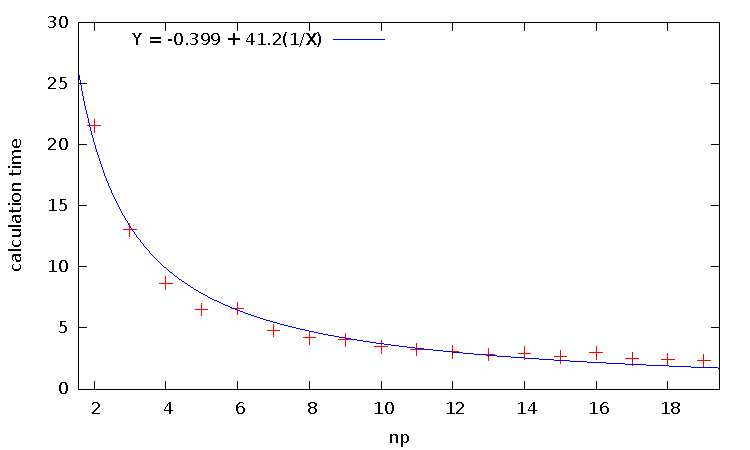
\includegraphics[scale=0.8]{figures/gamma-inverse}
  \caption{Gamma MLE script: calculation time versus number of
    processes with inverse fit}
  \label{fig:gamma-inverse}
\end{figure}

A second set of timings was obtained with the hosts file revised to
specify 4 slots per blade, thus invoking
hyper-threading. Figure~\ref{fig:gamma-log} compares the results with
and without hyper-threading, in the form of a log--log plot. It is
apparent that hyper-threading is not advantageous in this context.  In
fact the calculation time with $np=19$ and no hyper-threading (2.339
seconds) is much better than the minimum time with hyper-threading
(4.018 seconds at $np=33$).

\begin{figure}[htbp]
  \centering
  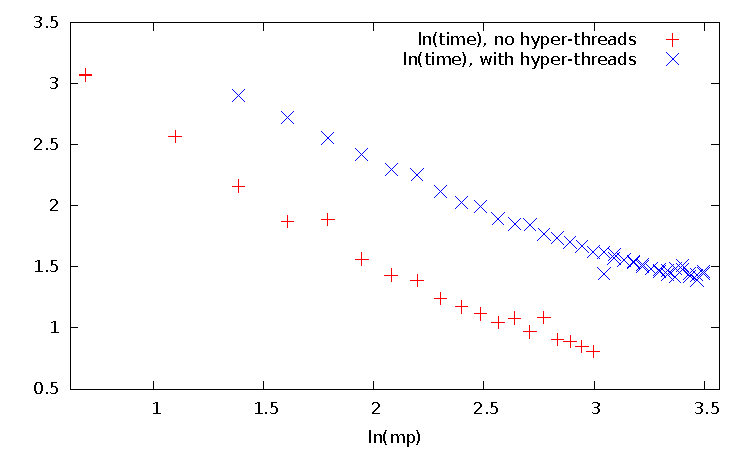
\includegraphics[scale=0.8]{figures/gamma-log}
  \caption{Gamma MLE script: log of calculation time versus log of
    number of processes, with and without hyper-threading}
  \label{fig:gamma-log}
\end{figure}

\end{document}

